\documentclass[aspectratio=169,11pt]{beamer}
% ==========================================================================
%  KSA lecture-slide theme  =  stock beamer "Boadilla"  +  KSA colour theme
%  brand colours sampled from the official KSA symbol mark:
%    Deep Prussian Blue  #2E3192   (지성 - intellect)
%    Golden Gray         #D6CBB1   (감성 - sensibility)
%  Engine: XeLaTeX.  Usage:
%    \documentclass[aspectratio=169,11pt]{beamer}
%    \input{../../theme/ksa-theme.tex}
%  Each deck lives in its own slides/kor/<deck>/ folder together with its
%  own images; ../../figs/ is kept only as a fallback for the shared cache.
% ==========================================================================

\usepackage{fontspec}
\usepackage{amsmath,amssymb}
\usepackage{graphicx}
\graphicspath{{figs/}{./}{../../../figs/}}
\usepackage{booktabs}
\usepackage{listings}
\usepackage{varwidth}

% ---- fonts (no ctex/xeCJK on this box -> fontspec drives CJK directly) -----
\defaultfontfeatures{Ligatures=TeX}
\setmainfont{Noto Sans CJK KR}
\setsansfont{Noto Sans CJK KR}
\setmonofont{Noto Sans Mono CJK KR}[Scale=0.92]

% ---- base theme: stock Boadilla ------------------------------------------
\usetheme{Boadilla}
\usefonttheme{professionalfonts}
\setbeamertemplate{navigation symbols}{}

% ---- KSA colour theme (recolour the stock theme) --------------------------
\definecolor{ksablue}{HTML}{2E3192}
\definecolor{ksabluedk}{HTML}{20226A}
\definecolor{ksagold}{HTML}{D6CBB1}
\definecolor{ksagolddk}{HTML}{A9976B}
\definecolor{ksared}{HTML}{C0392B}
\definecolor{ksagray}{HTML}{5B5B5B}

\setbeamercolor{structure}{fg=ksablue}
\setbeamercolor{alerted text}{fg=ksared}

\setbeamercolor{palette primary}{fg=white,           bg=ksablue}
\setbeamercolor{palette secondary}{fg=white,         bg=ksablue!85!black}
\setbeamercolor{palette tertiary}{fg=white,          bg=ksabluedk}
\setbeamercolor{titlelike}{fg=ksablue}
\setbeamercolor{frametitle}{fg=ksablue,bg=}
\setbeamercolor{title}{fg=ksablue}
\setbeamercolor{author}{fg=ksagray}
\setbeamercolor{institute}{fg=ksagray}
\setbeamercolor{block title}{fg=white,bg=ksablue}
\setbeamercolor{block body}{fg=black!85,bg=ksablue!6}
\setbeamercolor{item}{fg=ksablue}
\setbeamercolor{section in toc}{fg=black!85}

\setbeamerfont{frametitle}{series=\bfseries}
\setbeamerfont{title}{series=\bfseries}

% ---- footline:  KSA mark | "Made by ..." | n / N   (matches reference) ----
\newcommand{\ksacredit}{}
\setbeamertemplate{footline}{%
  \hbox{%
    \begin{beamercolorbox}[wd=.18\paperwidth,ht=2.6ex,dp=1.5ex,leftskip=1.1em]{}%
      \raisebox{-0.35ex}{\includegraphics[height=2.0ex]{ksa-logo.png}}%
    \end{beamercolorbox}%
    \begin{beamercolorbox}[wd=.64\paperwidth,ht=2.6ex,dp=1.5ex,center]{}%
      {\scriptsize\color{ksagray}\ksacredit}%
    \end{beamercolorbox}%
    \begin{beamercolorbox}[wd=.18\paperwidth,ht=2.6ex,dp=1.5ex,rightskip=1.1em]{}%
      \hfill{\scriptsize\color{ksablue}\insertframenumber\,/\,\inserttotalframenumber}%
    \end{beamercolorbox}%
  }%
  \vskip2pt
}

% ---- section divider: stock \sectionpage, KSA-coloured -------------------
\setbeamertemplate{section page}{%
  \begingroup\centering
    {\color{ksagolddk}\rule{0.16\paperwidth}{1pt}}\par\vskip1.0em
    {\usebeamerfont{title}\color{ksablue}\insertsectionhead\par}\vskip1.0em
    {\color{ksagolddk}\rule{0.16\paperwidth}{1pt}}\par
  \endgroup
}
\AtBeginSection[]{\begin{frame}[plain,noframenumbering]\vfill\sectionpage\vfill\end{frame}}

% ---- code listings ------------------------------------------------------------
\lstdefinestyle{ksa}{%
  basicstyle=\ttfamily\scriptsize,
  keywordstyle=\color{ksablue}\bfseries,
  commentstyle=\color{ksagray}\itshape,
  stringstyle=\color{ksagolddk},
  numberstyle=\tiny\color{ksagray},
  backgroundcolor=\color{ksablue!6},
  frame=leftline, framerule=1.4pt, rulecolor=\color{ksablue},
  xleftmargin=1em, aboveskip=0.8em, belowskip=0.4em,
  showstringspaces=false, breaklines=true, language=Python,
}
\lstset{style=ksa}

% ---- handy macros -----------------------------------------------------------
\newcommand{\kb}[1]{\textbf{\color{ksablue}#1}}   % blue keyword
\newcommand{\kq}[1]{\textbf{\color{ksared}#1}}    % red key-question

\setbeamerfont{title}{series=\bfseries,size=\fontsize{24}{30}\selectfont}
\setbeamerfont{subtitle}{series=\bfseries,size=\fontsize{14}{18}\selectfont}
\setbeamerfont{author}{size=\normalsize}
\setbeamerfont{institute}{size=\small}
\graphicspath{{figs/}{../../../../assets/}}
\makeatletter
\newcommand{\markpage}[1]{\protected@write\@auxout{}{\string\newlabel{#1}{{\the\c@framenumber}{}}}\hypertarget{#1}{}}
\newcommand{\pref}[1]{\hyperlink{#1}{\textcolor{ksagolddk}{(p.\ref{#1})}}}
\makeatother

\renewcommand{\ksacredit}{Machine Learning 1 \,\textperiodcentered\, kNN 최근접 이웃}
\title{kNN 최근접 이웃 (k-Nearest Neighbors)}
\subtitle{가장 가까운 k개에게 물어보기, 그리고 차원의 저주}
\author{Machine Learning 1}
\institute{한국과학영재학교 (KSA)}
\date{}
\begin{document}
\begin{frame}[plain,noframenumbering]\titlepage\end{frame}

% --- 오늘의 질문
\begin{frame}{오늘의 질문}
\vfill
\centering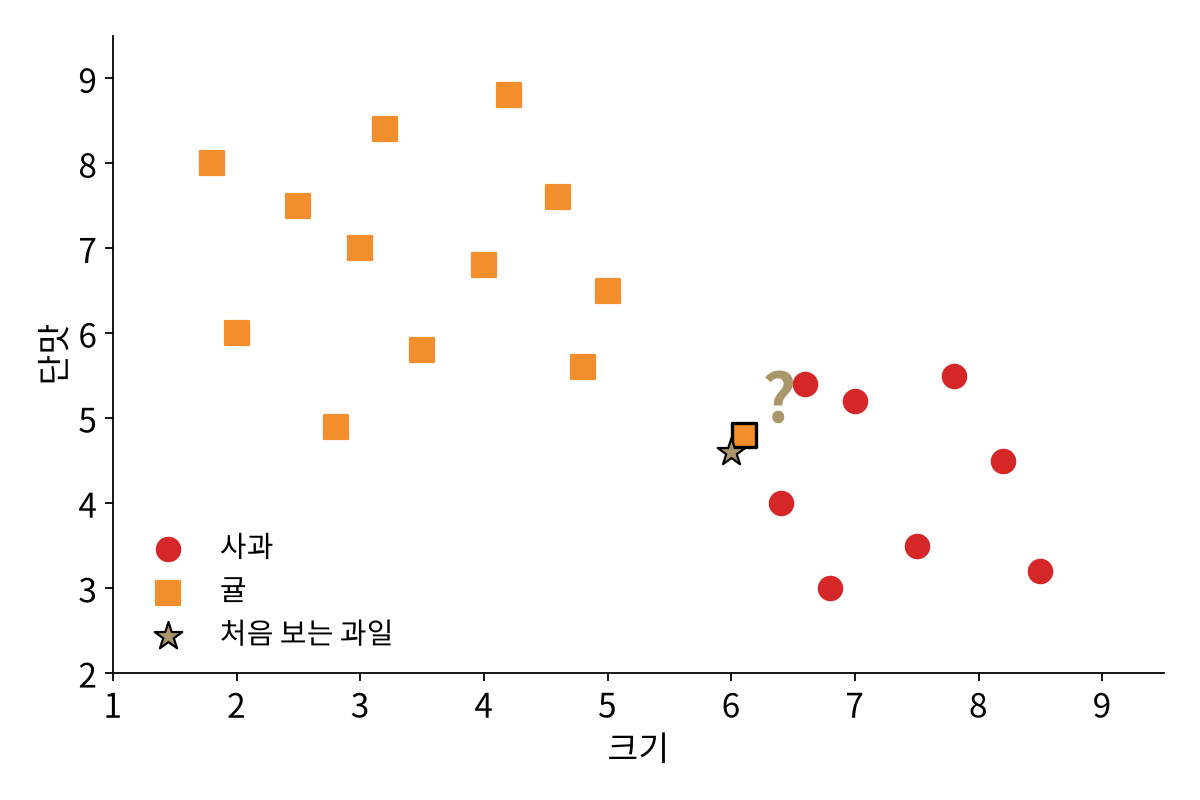
\includegraphics[width=0.56\linewidth]{kn_hook.png}\par\vskip0.2em
{\large 크기와 단맛을 잰 과일 21개. \kq{처음 보는 과일 (별) 은 사과일까, 귤일까?}}
\vfill
\note{과일 21개의 크기와 단맛을 재서 점으로 찍었습니다. 빨간 동그라미가 사과, 주황 네모가 귤입니다. 사과는 크고 덜 달고, 귤은 작고 더 답니다. 노란 별은 처음 보는 과일입니다. 사과일까요, 귤일까요? 공식을 몰라도 사람은 이렇게 답합니다. 주변에 사과가 많으니 사과겠지. 오늘 배울 kNN은 바로 이 생각을 그대로 알고리즘으로 만든 것입니다.}
\end{frame}

% --- k=3
\begin{frame}{가장 가까운 3개에게 묻기}
\markpage{k3}
\vfill
\begin{columns}[c]
\begin{column}{0.5\textwidth}\centering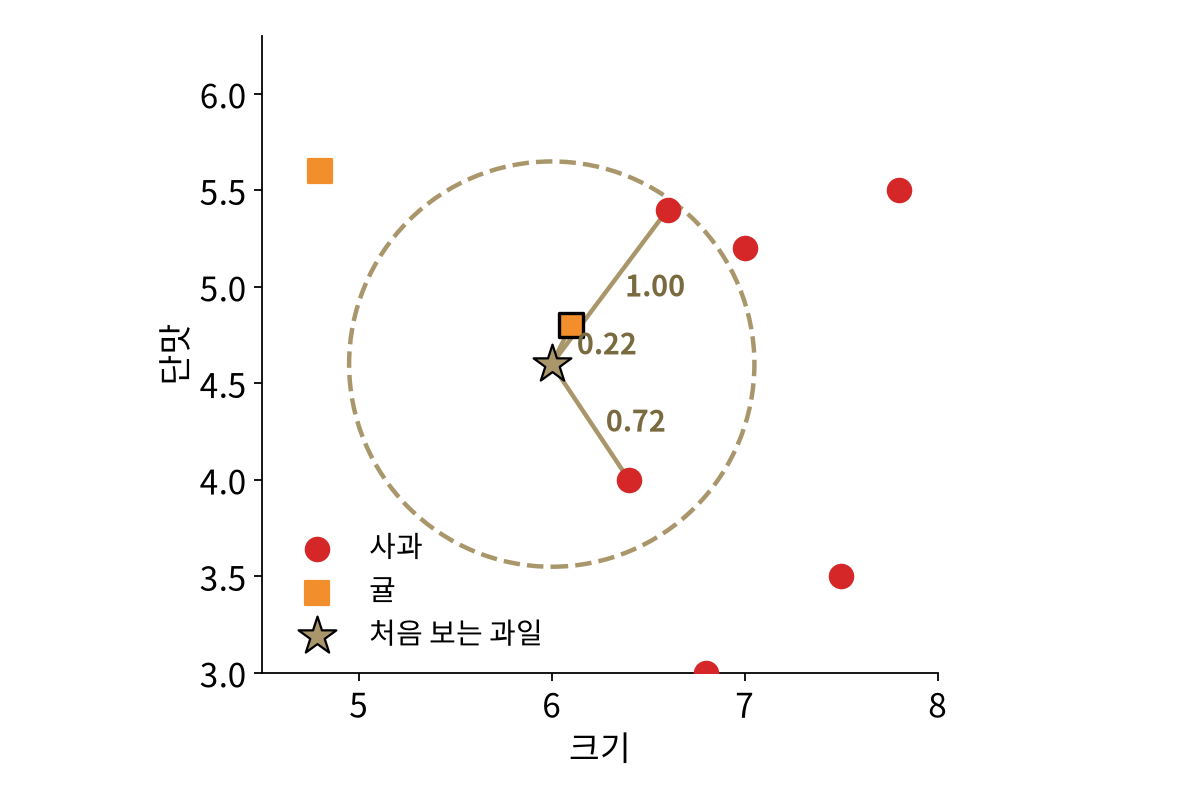
\includegraphics[width=\linewidth]{kn_k3.png}\end{column}
\begin{column}{0.46\textwidth}
{\large $k = 3$: 가장 가까운 3개}\\[0.6em]
{\large 귤 1 · 사과 2}\\[0.6em]
{\Large $\to$ 다수결로 \kq{사과}}\\[1em]
{\small kNN = k-Nearest Neighbors\\ (k-최근접 이웃)}
\end{column}
\end{columns}
\vfill
\note{별에서 가장 가까운 과일 3개를 찾습니다. 숫자는 별까지의 거리입니다. 0.22에 귤 하나, 0.72와 1.0에 사과 둘이 있습니다. 3개 중 사과가 2개이니 다수결로 사과라고 답합니다. 이것이 kNN, k 최근접 이웃의 전부입니다. k는 몇 개의 이웃에게 물어볼지를 정하는 숫자입니다.}
\end{frame}

% --- 거리
\begin{frame}{``가깝다'' = 유클리드 거리}
\vfill
\centering
{\LARGE\[ d(\mathbf{x}, \mathbf{q}) = \sqrt{\sum_{j=1}^{n} (x_j - q_j)^2} \]}\vskip0.4em
{\large 별 $(6.0,\ 4.6)$ 과 사과 $(6.4,\ 4.0)$: \quad $\sqrt{(6.4 - 6.0)^2 + (4.0 - 4.6)^2} = \sqrt{0.16 + 0.36} = 0.72$}\\[0.8em]
{\small $n$: 특징 수 (지금은 크기 · 단맛, 2개) \qquad 특징이 몇 개든 같은 식}
\vfill
\note{가깝다는 것은 보통 유클리드 거리, 즉 자로 잰 직선 거리입니다. 특징마다 차이를 제곱해서 더하고 루트를 씌웁니다. 별은 크기 6.0, 단맛 4.6이고, 가장 가까운 사과는 6.4와 4.0입니다. 차이는 0.4와 마이너스 0.6, 제곱하면 0.16과 0.36, 더하면 0.52, 루트를 씌우면 0.72입니다. 특징이 10개, 100개가 되어도 같은 식으로 잽니다. 이 점이 나중에 차원의 저주에서 문제가 됩니다.}
\end{frame}

% --- 학습 없음
\begin{frame}{학습이 없는 학습}
\vfill
\centering
\renewcommand{\arraystretch}{1.5}
{\large\begin{tabular}{rl}
\textbf{학습} & 데이터를 \kb{외워 두기만} 한다 \quad (가중치도, 경사하강법도 없다)\\
\textbf{예측} & \textcircled{1} 모든 점과 거리 재기 \; \textcircled{2} 가까운 순 정렬 \; \textcircled{3} 앞의 $k$ 개 다수결
\end{tabular}}\vskip1.0em
{\large 데이터 $m$ 개, 특징 $n$ 개 $\to$ 예측 한 번에 거리 계산 $m$ 번 (각각 $n$ 개 더하기)}\\[0.4em]
{\small 선형회귀는 학습이 느리고 예측이 빠르다. kNN 은 반대: \kq{비용이 예측할 때 몰린다}}
\vfill
\note{kNN에는 학습 단계가 사실상 없습니다. 선형회귀처럼 가중치를 찾지도, 경사하강법을 돌리지도 않습니다. 데이터를 외워 두기만 합니다. 대신 예측할 때마다 모든 점과 거리를 재고, 가까운 순으로 정렬해서, 앞의 k개로 다수결을 냅니다. 데이터가 m개면 예측 한 번에 거리를 m번 재야 합니다. 선형회귀는 학습이 오래 걸리지만 예측은 곱하기 몇 번이면 끝나는데, kNN은 반대로 비용이 예측 때 몰립니다. 데이터가 수백만 개면 이게 큰 문제가 되고, 그래서 가까운 점을 빨리 찾는 자료구조가 따로 연구됩니다.}
\end{frame}

% --- k 의 영향
\begin{frame}{$k$ 가 너무 작거나 너무 크면}
\markpage{boundary}
\vfill
\centering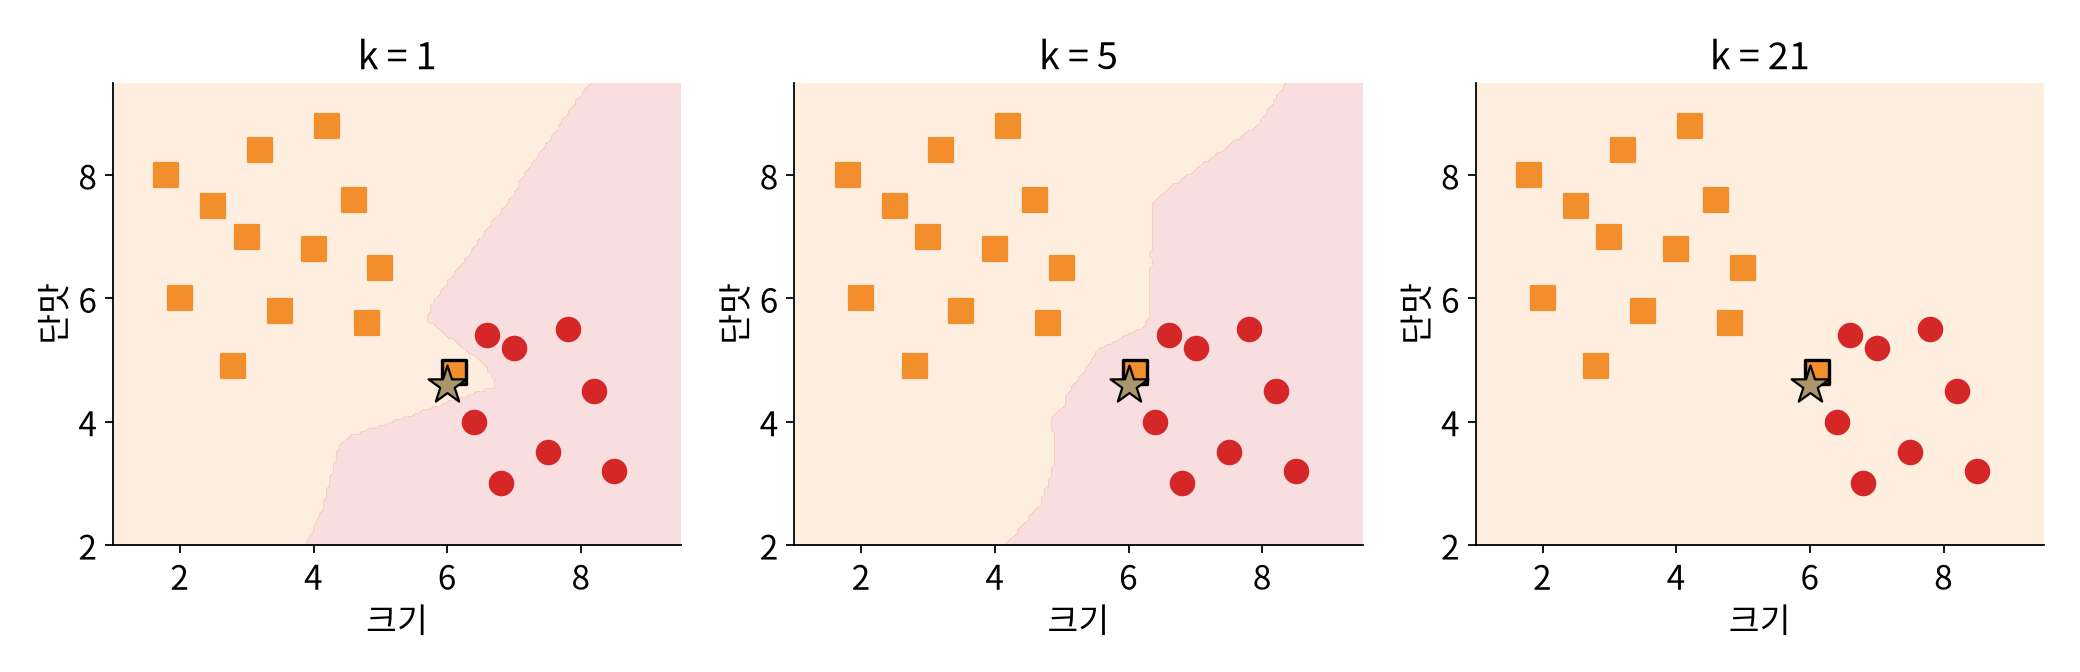
\includegraphics[width=0.96\linewidth]{kn_boundary.png}\par\vskip0.2em
{\large $k = 1$: 잘못 적힌 귤 (검은 테두리) 하나에 속는다 \quad $k = 21$: 전체 다수결 $\to$ \kq{늘 귤}}
\vfill
\note{배경색은 그 위치에 새 과일이 오면 어떻게 답할지를 칠한 것입니다. k가 1이면 가장 가까운 하나만 봅니다. 사과 무리 한가운데 귤로 잘못 적힌 점, 검은 테두리 네모가 있는데, 그 주변이 통째로 귤이 되어 버립니다. 별도 이 점 바로 옆이라 귤이라고 답합니다. 데이터의 실수까지 외우는 과대적합입니다. 반대로 k가 21, 전체 데이터면 언제나 전체의 다수결이니 귤 13개, 사과 8개로 어디서든 귤입니다. 너무 단순한 과소적합입니다. 가운데 k가 5일 때 경계가 가장 자연스럽습니다.}
\end{frame}

% --- k 고르기
\begin{frame}{$k$ 는 검증으로 고른다}
\vfill
\centering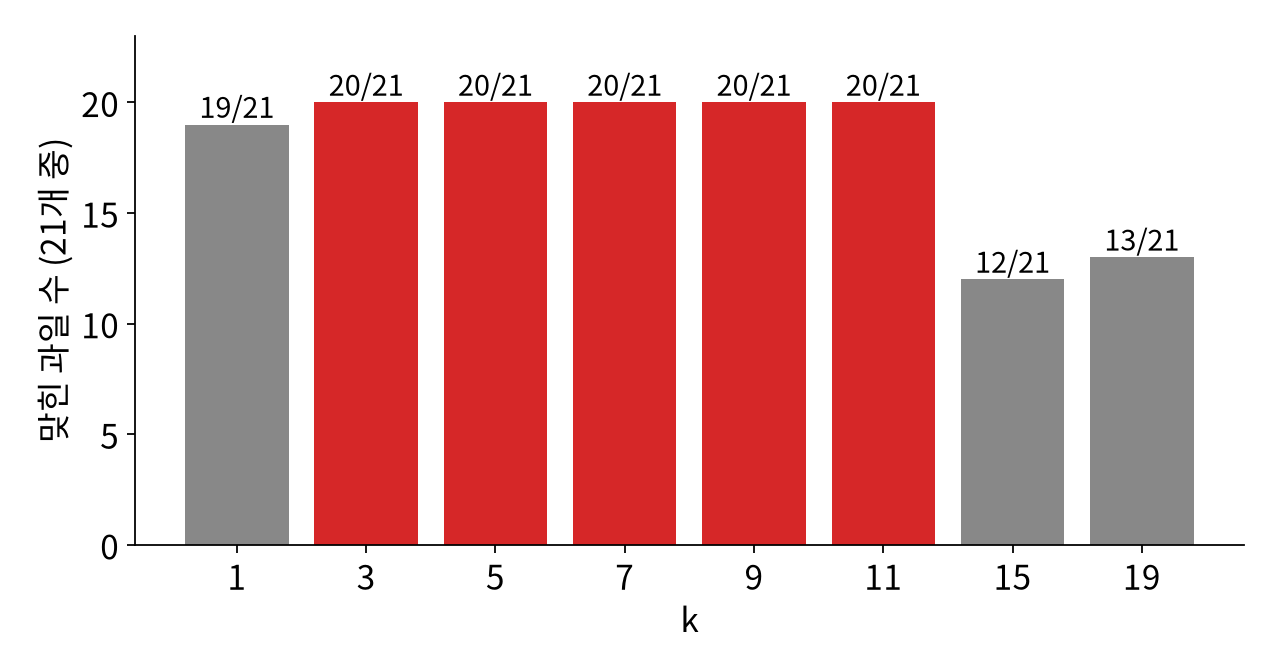
\includegraphics[width=0.56\linewidth]{kn_loo.png}\par\vskip0.2em
{\large 하나씩 빼 두고 나머지 20개로 맞혀 보기 \quad $k = 3 \sim 11$ 이 \kb{20/21}}\\[0.2em]
{\small leave-one-out: 조각 크기가 1 인 교차 검증}
\vfill
\note{그러면 k는 어떻게 고를까요? 과대적합 시간에 배운 교차 검증을 씁니다. 데이터가 21개뿐이라 하나씩 숨겨 봅니다. 과일 하나를 빼 두고 나머지 20개로 kNN을 해서 맞히는지 보고, 21번 반복합니다. k가 1이면 21개 중 19개를 맞히는데, 3부터 11까지는 20개를 맞힙니다. 15를 넘으면 귤이 너무 많아져서 12개, 13개로 무너집니다. 이렇게 하나씩 빼는 교차 검증을 leave-one-out이라고 합니다. 동점이면 보통 작은 k가 계산이 빠르고, 이진 분류에서는 동점 투표가 안 나오게 홀수를 씁니다.}
\end{frame}

% --- 단위
\begin{frame}{단맛을 100 점 만점으로 재면?}
\markpage{scale}
\vfill
\centering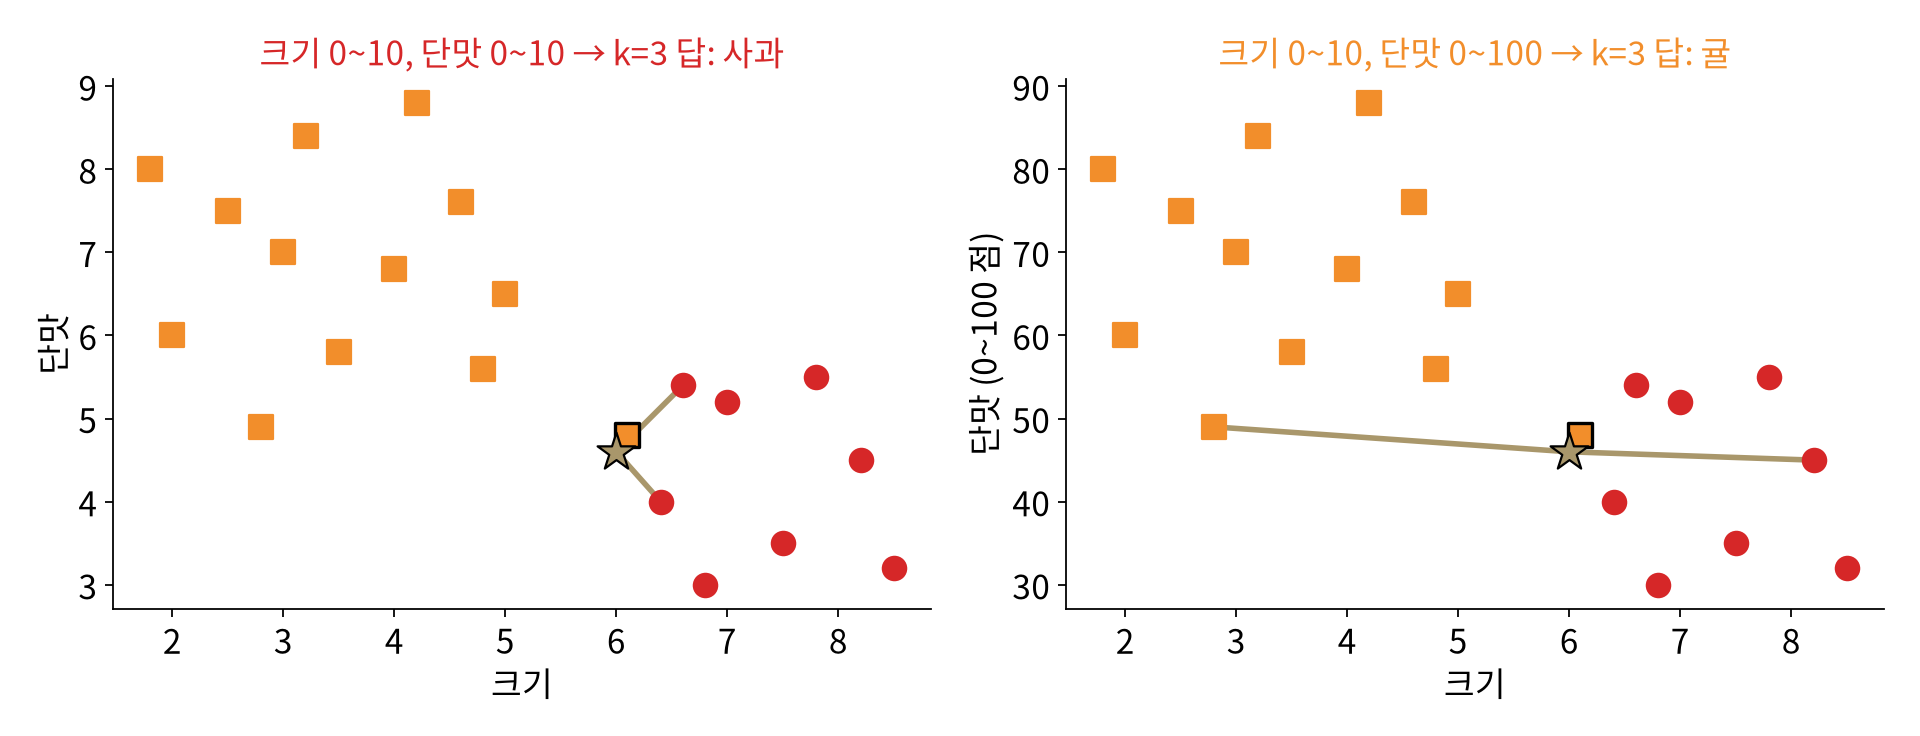
\includegraphics[width=0.86\linewidth]{kn_scale.png}\par\vskip0.2em
{\large 단위만 바꿨는데 $k = 3$ 의 답이 \kq{귤}로 \quad 거리를 \textbf{단맛}이 혼자 정한다}
\vfill
\note{단맛을 0에서 10이 아니라 100점 만점으로 재면 어떻게 될까요? 과일은 똑같고 단위만 바꿨습니다. 그런데 이제 단맛 차이는 10배가 되어서 거리를 거의 혼자 정합니다. 크기 차이는 무시되고, 단맛이 비슷한 과일만 가깝게 보입니다. 그 결과 k가 3일 때 가까운 이웃이 귤 둘, 사과 하나로 바뀌고 답이 귤이 됩니다. 단위를 바꿨을 뿐인데 답이 바뀐 겁니다.}
\end{frame}

% --- 표준화
\begin{frame}{해결: 특징마다 같은 목소리 (표준화)}
\vfill
\centering
{\LARGE\[ z_j = \frac{x_j - \mu_j}{\sigma_j} \]}\vskip0.4em
{\large 특징마다 평균 0, 표준편차 1 로 맞춘 뒤 거리를 잰다 \quad (가우시안 시간의 $z$ 점수)}\\[0.8em]
{\large 실제 데이터 (와인 178병, 특징 13개): \; 그대로 \textbf{71\%} \quad 표준화 후 \kb{97\%} \quad ($k = 5$)}\\[0.4em]
{\small 와인 데이터에서 프롤린은 수백 $\sim$ 1,600, 색 농도는 1 $\sim$ 13 $\to$ 그대로 두면 프롤린 하나가 거리를 정한다}
\vfill
\note{해결책은 표준화입니다. 특징마다 평균을 빼고 표준편차로 나눠서, 모든 특징을 평균 0, 표준편차 1로 맞춥니다. 가우시안 시간의 z 점수와 같은 식입니다. 그러면 단위와 상관없이 모든 특징이 같은 크기의 목소리를 냅니다. 실습에서 쓸 와인 데이터는 와인 178병의 화학 성분 13개로 품종 셋을 맞히는 문제입니다. 그대로 kNN을 하면 71퍼센트인데, 표준화하면 97퍼센트가 됩니다. 프롤린이라는 성분은 수백에서 1600까지인데 다른 성분은 1에서 13 정도라서, 그대로 두면 프롤린 하나가 거리를 정해 버리기 때문입니다.}
\end{frame}

% --- 차원의 저주 1
\begin{frame}{차원의 저주: 가까운 이웃이 사라진다}
\vfill
\centering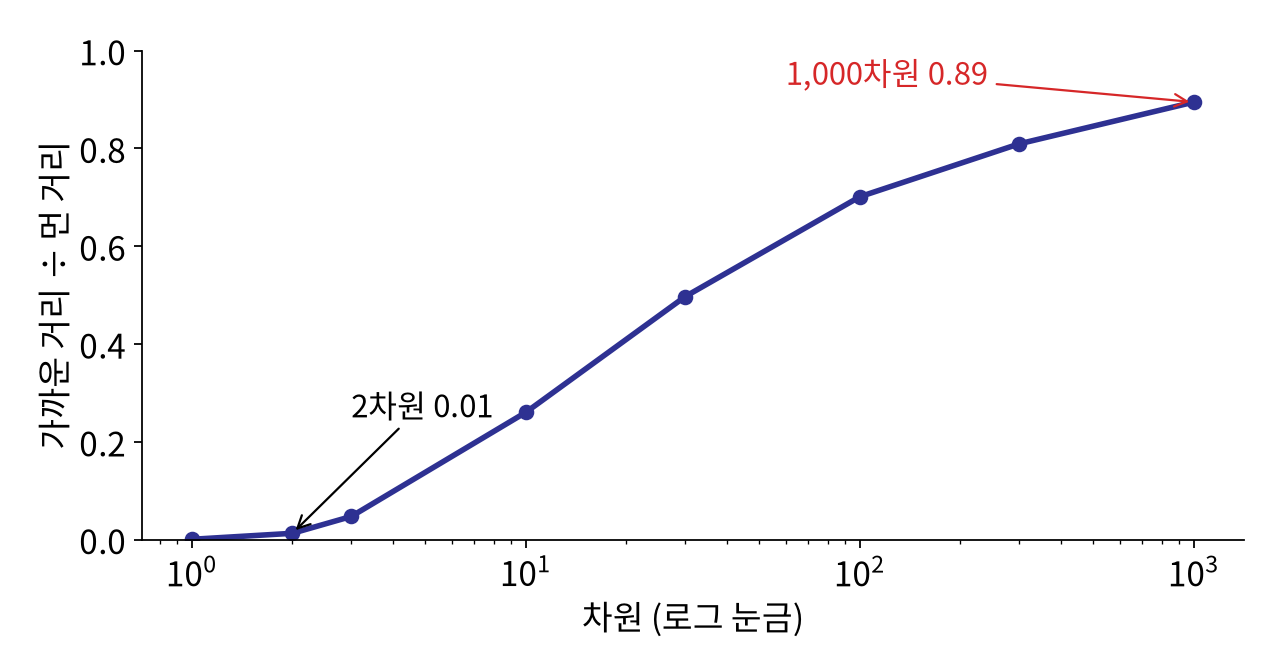
\includegraphics[width=0.56\linewidth]{kn_ratio.png}\par\vskip0.2em
{\large 가장 가까운 거리 $\div$ 가장 먼 거리 (점 1,000개): \quad 2차원 \kb{0.01} $\to$ 1,000차원 \kq{0.9}}\\[0.2em]
{\small 차원이 높으면 가장 가까운 점도 가장 먼 점만큼 멀다 \quad Curse of Dimensionality (Bellman, 1957)}
\vfill
\note{특징이 많아지면 kNN에는 더 근본적인 문제가 생깁니다. 정육면체 안에 점 1000개를 균등하게 뿌리고, 한 점에서 가장 가까운 점까지의 거리를 가장 먼 점까지의 거리로 나눠 봤습니다. 2차원에서는 0.01, 가까운 점은 정말 가깝습니다. 그런데 차원을 올릴수록 이 비율이 1에 가까워져서 1000차원에서는 0.9입니다. 가장 가까운 점도 가장 먼 점과 거의 같은 거리에 있다는 뜻입니다. 그러면 가장 가까운 이웃이라는 말 자체가 의미를 잃습니다. 이 현상을 차원의 저주라고 하고, 1957년 벨만이 붙인 이름입니다.}
\end{frame}

% --- 차원의 저주 2
\begin{frame}{뜻 없는 특징을 더하면}
\vfill
\centering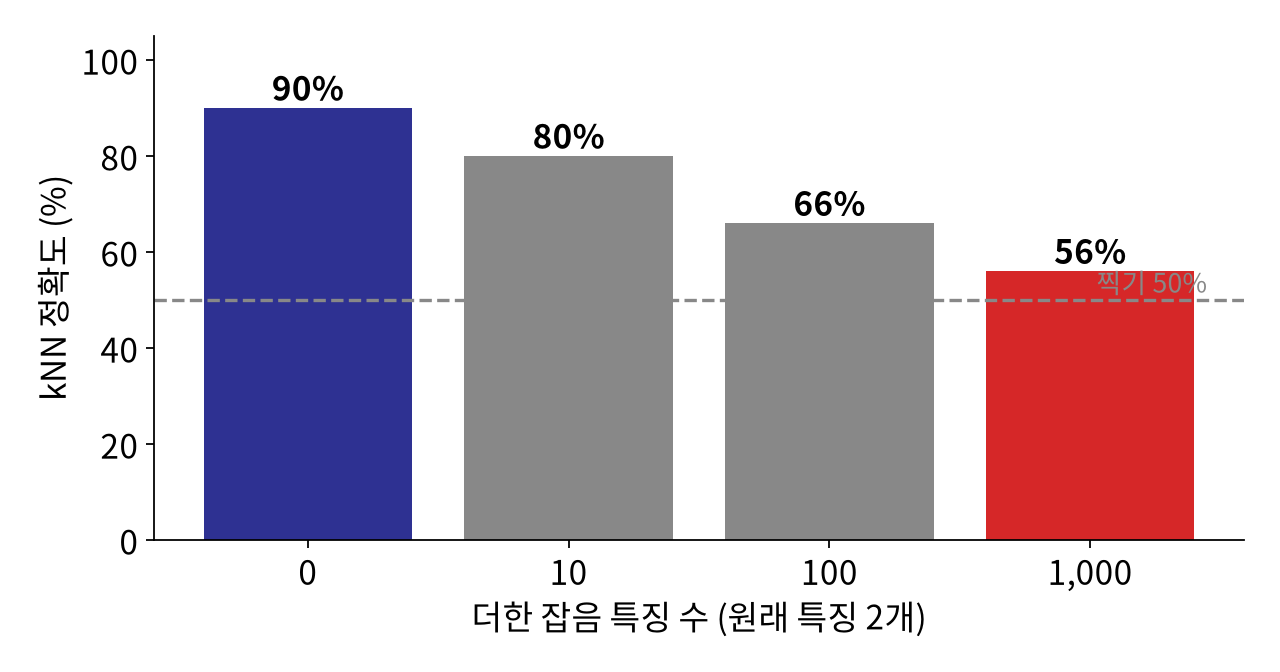
\includegraphics[width=0.56\linewidth]{kn_noise.png}\par\vskip0.2em
{\large 두 반달 데이터 (특징 2개) 에 난수 특징을 더하면 \quad 90\% $\to$ 80 $\to$ 66 $\to$ \kq{56\%}}\\[0.2em]
{\small 특징은 많을수록 좋은 게 아니다 $\to$ 쓸모 있는 특징만 고르거나, 차원을 줄인다 (14주차 PCA)}
\vfill
\note{실제로 얼마나 나빠질까요? 두 반달 모양으로 나뉜 데이터는 특징 2개만으로 kNN 정확도가 90퍼센트입니다. 여기에 아무 뜻 없는 난수 특징을 10개 더하면 80퍼센트, 100개면 66퍼센트, 1000개면 56퍼센트로 거의 찍기 수준이 됩니다. 원래의 유용한 두 특징은 그대로 있는데도요. 뜻 없는 축의 거리가 쌓여서 진짜 차이를 덮어 버리기 때문입니다. 그래서 특징은 많을수록 좋은 게 아닙니다. 쓸모 있는 특징만 고르거나, 14주차에 배울 PCA처럼 차원을 줄인 뒤에 거리를 잽니다.}
\end{frame}

% --- 문제풀이
\begin{frame}{문제풀이}
\vfill
\begin{enumerate}
\item 점 A $(1, 1)$ 사과, B $(2, 3)$ 귤, C $(4, 1)$ 사과, D $(3, 4)$ 귤. 새 점 $(2, 2)$ 에 대해 (a) 네 거리는? \; (b) $k = 1$, $k = 3$ 의 답은?\vskip0.8em
\item 학습 데이터 100만 개로 kNN 과 선형회귀를 만들었다. 예측 한 번이 더 오래 걸리는 쪽은? 이유는?\vskip0.8em
\item 키 (cm) 와 몸무게 (kg) 로 kNN 을 한다. 키를 mm 로 바꾸면 무슨 일이 생기나? 어떻게 막나?\vskip0.8em
\item 특징 2개로 90\% 이던 kNN 에 특징을 50개 더했더니 70\% 가 됐다. 무엇을 의심해야 하나?
\end{enumerate}
\vfill
\note{1번 답. A까지 루트 2, 약 1.41, B까지 1, C까지 루트 5, 약 2.24, D까지 루트 5, 약 2.24입니다. k가 1이면 가장 가까운 B, 귤입니다. k가 3이면 B와 A, 그리고 C와 D가 같은 거리라서 동점입니다. 동점 처리 규칙이 필요하다는 게 답의 핵심이고, 예를 들어 먼저 나온 C를 쓰면 사과 2, 귤 1로 사과입니다. 2번 답. kNN입니다. 예측할 때마다 100만 개와 거리를 재야 하니까요. 3번 답. 키 차이가 10배가 되어 거리를 키가 혼자 정합니다. 표준화로 막습니다. 4번 답. 차원의 저주입니다. 더한 특징이 쓸모없는 잡음일 가능성을 의심하고, 특징을 골라 봅니다.}
\end{frame}

% --- 실습
\begin{frame}{실습}
\vfill
\centering\begin{tabular}{rl}
\large 1 & kNN 직접 구현: 거리 · 정렬 · 다수결 $\to$ 슬라이드의 과일로 $k = 1, 3, 21$ 재현\\[0.5em]
\large 2 & 실제 데이터: 와인 178병, 표준화 전후 비교 (71\% $\to$ 97\%)\\[0.5em]
\large 3 & 교차 검증으로 $k$ 고르기 + 잡음 특징을 더하며 차원의 저주 보기
\end{tabular}\vskip1em
Wine (Forina et al.; UCI) \\[0.4em]\href{https://colab.research.google.com/github/SuminHan/book-ml/blob/main/slides/v2/ml1/week04/knn/lab/knn.ipynb}{\textcolor{ksagolddk}{▶ Colab에서 실습 노트북 열기}}
\vfill
\note{실습은 세 부분입니다. 첫째, 거리 재기, 정렬, 다수결 세 단계를 직접 구현해서 슬라이드의 과일로 k가 1, 3, 21일 때 답을 재현합니다. 둘째, 실제 와인 데이터로 표준화를 하기 전과 후를 비교합니다. 셋째, 교차 검증으로 k를 고르고, 잡음 특징을 더해 가며 정확도가 어떻게 무너지는지 직접 봅니다.}
\end{frame}

% --- 정리
\begin{frame}{정리}
\vfill
\centering\large\begin{tabular}{l}
\textbf{kNN} \quad 가장 가까운 $k$ 개의 다수결 \quad 학습 없이 외우고, 예측 때 거리를 잰다\\[0.5em]
$k$ 가 작으면 과대적합, 크면 과소적합 $\to$ \textbf{교차 검증}으로 고른다\\[0.5em]
단위가 다르면 거리가 왜곡된다 $\to$ \kb{표준화} 먼저\\[0.5em]
특징이 많으면 이웃이 사라진다 $\to$ \kq{차원의 저주}
\end{tabular}
\vfill
\note{정리합니다. kNN은 가장 가까운 k개의 다수결입니다. 학습 단계 없이 데이터를 외워 두고, 예측할 때마다 거리를 잽니다. k가 작으면 잡음까지 외우는 과대적합, 크면 늘 많은 쪽만 답하는 과소적합이라 교차 검증으로 고릅니다. 특징의 단위가 다르면 거리가 왜곡되니 표준화를 먼저 하고, 특징이 너무 많으면 차원의 저주로 가까운 이웃이라는 개념 자체가 무너집니다. 다음 시간에는 정답 라벨 없이 데이터를 무리로 나누는 k-means를 배웁니다.}
\end{frame}
\end{document}
